\documentclass[11pt]{article}
% General document formatting
\usepackage[margin=0.75in]{geometry}
\usepackage[parfill]{parskip}
\usepackage[utf8]{inputenc}
\usepackage{subfig}         % side-by-side figures 
% Related to math
\usepackage{amsmath,amssymb,amsfonts,amsthm}
\usepackage{graphicx}
\usepackage{natbib}
\usepackage{titling}
\usepackage{hyperref}
\usepackage{wrapfig}
\usepackage{booktabs} % for wrapping tabulars in accord with
\bibliographystyle{agu}
\setlength{\droptitle}{-5em}   % This is your set screw

%\usepackage[math]{kurier}
\newcommand\be{\begin{equation}} % shortcut to start eq envs 
\newcommand\ee{\end{equation}}   % shortcut to end eq envs
\newcommand\ol{\overline}        % shortcut to draw overline 
\newcommand\bra{\langle}
\newcommand\ket{\rangle}
\newcommand\El{\mathcal{L}}
\newcommand\tg{\tilde{g}}
\newcommand\tG{\tilde{G}}
\begin{document}

\title{Bedload diffusion theory}
\author{Kevin Pierce}
\maketitle

\section{The two-state random walk}
The formalism of two-state random walks \citep[e.g.][]{Weiss1976,Weiss1994,Masoliver2016,Masoliver2017} ultimately composes all existing models of bedload diffusion \citep[e.g.][]{Nikora2001a,Nikora2002,Zhang2012,Fan2016} and provides a framework to build new models from.
Assuming residence time distributions $\psi_i(t)$ in the states with associated survival probabilities $\Psi_i(t) = \int_t^\infty dt' \psi_i(t')$, probabilities of moving a distance $x$ up to time $t$ within a sojourn $f_i(x,t)$, denoting $g_i(x,t) =f_i(x,t)\psi_i(t)$ and $G_i(x,t) = f_i(x,t)\Psi_i(x,t)$, and letting $\omega_i(x,t)$ be the probability that a sojourn in state $i$ ends at $x,t$ provides
\be  p_i(x,t) = \theta_i G_i(x,t) + \int_0^\infty dx' \int_0^\infty dt' \omega_{\bar{i}}(x',t')G_i(x-x',t-t')\ee
and 
\be \omega_i(x,t) = \theta_i g_i(x,t) + \int_0^\infty dx' \int_0^\infty dt' \omega_{\bar{i}}(x',t')g_i(x-x',t-t').\label{eq:two}\ee
Here $\theta_i$ are the initial probabilities of being in each state with $\theta_1 + \theta_2=1.$ $\bar{i}$ is the opposite of $i$ and $i=1,2$.
The probability of the two-state random walker being at position $x$ at time $t$ is 
\be p(x,t) = p_1(x,t)+p_2(x,t).\ee
Denoting the laplace transform with respect to the variable $q$ as $\El_q$ and associating variables $\eta$ and $s$ with $\El_x$ and $\El_t$, 
taking $\El_x \El_t$ of (\ref{eq:two}) provides a much simpler algebraic problem for the probability $p$:

\be
\tilde{\omega}_i = 
\frac{[\theta_i+ \theta_{\bar{i}} \tilde{g}_{\bar{i}}]\tilde{g}_i}{1-\tilde{g}_1\tilde{g}_2}
\ee
and (c.f. \citet{Masoliver2016} eq. 20)
\be
\tilde{p}_\pm = \Big( \theta_i + \tilde{\omega}_{\bar{i}} \Big)\tilde{G}_i = \frac{\theta_i + \theta_{\bar{i}} \tilde{g}_{\bar{i}}}{1- \tilde{g}_1\tilde{g}_2}\tilde{G}_i.
\ee
Therefore the double transform of the joint PDF reads \citep[c.f.][eq. 6.33 pg. 243]{Weiss1994}
\be
\tilde{p}(\eta,s) = \frac{\theta_1[\tilde{G}_1 + \tilde{g}_1 \tilde{G}_2] + \theta_2[\tilde{G}_2 + \tilde{g}_2 \tilde{G}_1]}{1-\tilde{g}_1 \tilde{g}_2}.
\label{eq:mw}\ee
This is a direct generalization of the famous Montroll-Weiss formula for a single state continuous-time random walk.

For the evaluation of this formula, a useful fact to take account of is 
\be \El_t\{ \Psi_\pm(t);s\} = \int_0^\infty dt e^{-st} \int_t^\infty dt' \psi_\pm(t') = \frac{1-\tilde{\psi}(s)}{s}. \ee
Finally, owing to the definition of the double Laplace transform of $p(x,t)$:
\be \tilde{p}(\eta,s) = \int_0^\infty dt e^{-st} \int_0^\infty dx e^{-\eta x} p(x,t)\ee
we see the (double) inverse transform $p(x,t)$ is not necessary to study the moments $\bra x(t)^k \ket = \int_0^\infty x^k p(x,t)$ of an ensemble of tracers since the moments follow from
\be \El_t\{\bra x(t)^k\ket;s\} = (-)^k\partial_\eta^k \tilde{p}(\eta,s)\Big|_{\eta=0}.\ee

\subsection{Moments of a two-state random walk}
\citet{Weeks1998} starts in motion, for future reference. 
In this section I will analyze the moments in generality.



\section{The Einstein theory}
Taking $g_1(x,t) = \delta(x)k_1 e^{-k_1t}$ (rest) and $g_2(x,t) = k_2 e^{-k_2 x}\delta(t) $ (step) reproduces the \citet{Einstein1937} diffusion theory.
In this case the double transforms are: 
\be \tilde{g}_1(\eta,s) = \frac{k_1}{k_1+s}\ee
\be \tilde{g}_2(\eta,s) = \frac{k_2}{k_2+\eta}, \ee
and the survival functions are 
\be \Psi_1(t) = \int_t^\infty dt' k_1e^{-k_1 t'} = e^{-k_1 t} \ee
and 
\be \Psi_2(t) = \int_t^\infty dt' \delta(t') = 0 ,  \ee
meaning $G_1(x,t) = \delta(x) e^{-k_1 t}$ and $G_2(x,t) = 0,$ providing
\be \tG_1(\eta,s) = \frac{1}{k_1+s}.\ee
Taking $\theta_1=1$ and $\theta_2=0$, so the dynamics start at rest, the MW generalization (\ref{eq:mw}) is
\be \tilde{p}(\eta, s) = \frac{\tG_1}{1-\tg_1\tg_2} = \frac{1}{s + \frac{k_1 \eta}{k_2 + \eta }}.\label{eq:mwgen}\ee
The Laplace transform of the mean is 
\be \bra \tilde{x} \ket = \frac{k_1}{s^2 k_2}
\ee
so in real space it's $\bra x \ket = k_- t/k_+$ as expected \citep[e.g.][]{Einstein1937, Nakagawa1976}.
The Laplace transform of the second moment is 
\be\bra \tilde{x}^2 \ket = 2\Big(\frac{k_1}{k_2}\Big)^2 \Big[ \frac{1}{k_1}\frac{1}{s^2} + \frac{1}{s^3}\Big], \ee
implying a second moment $\bra x^2 \ket = (k_1/k_2)^2[2t/k_1+t^2] $
and a variance exemplifying the normal diffusion of bedload:
\be \sigma_x^2 = \frac{2k_1}{k_2^2}t.\ee
This is depicted in figure \ref{fig:einwalk}.
\begin{figure}[h]
	\centering
	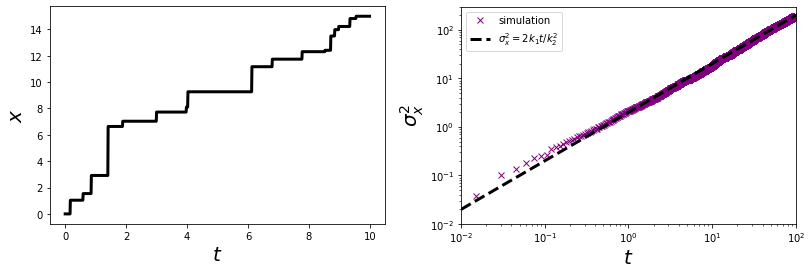
\includegraphics[width=\linewidth,keepaspectratio]{combo0.png}
	\caption{Left panel shows the Einstein walk in x-t space while the right panel shows the linear variance. There is a single range of normal diffusion when steps are instantaneous.}
	\label{fig:einwalk}
\end{figure}
Of course, for the Einstein theory a closed form solution of the pdf $p(x,t)$ is possible to obtain \citep[e.g.][]{Einstein1937, Hubbell1964, Daly2006,Daly2019}.
The first transform in (\ref{eq:mwgen}) inverts easily for 
\be \tilde{p}(\eta,t) = \exp\Big\{-\frac{k_1\eta }{k_2 + \eta} t\Big\}.\ee
Incidentally this single Laplace transform of $p$ provides the cumulant generating function $c(\eta,t) = \log \tilde{p}(-\eta,t)$ from which the variance follows from a more simple computation: $\sigma_x^2(t) = \partial_\eta^2 c(\eta,t)\big|_{\eta=0}.$
The second inversion gives \citep[e.g.][]{Daly2019}
\be p(x,t) = e^{-k_1 t -k_2 x}\Big\{ \sqrt{\frac{k_1 k_2 t}{ x}} I_1\Big( 2\sqrt{k_1k_2 x t}\Big) + \delta(x) \Big\} .\ee
This exact solution has been the benchmark theory of bedload diffusion for over 100 years. I have only derived it within a more general framework of multi-state random walks \citep[e.g.][]{Weiss1994}.

A final note -- taking the expression for $\tilde{p}(\eta,t)$ and inverting as in \citet{Weiss1994} pg. 247 gives the equation 
\be [k_1 \partial_x + k_2\partial_t + \partial_x \partial_t] p = 0, \ee
after some jangling.
I'm surprised this is not the normal diffusion equation.
I'm curious if it's correct and if the solution involving $I_1$ solves it.
Decomposing $p = e^{-k_1 t - k_2 x}\pi$ gives 
\be \partial_x \partial_t \pi = k_1 k_2\pi.\ee
Using the series representation 
\be \pi(x,t) = k_1k_2 \sum_{m=0}^\infty \frac{(k_1k_2)^m}{m!(m+1)!}t^{m+1}x^m \ee
it's possible to see that the solution given earlier satisfies this differential equation. Presumably this would also follow from the Frobenius method.
\section{The Lisle Theory}
Apart from formulations of \citet{Einstein1937} using different step length and resting time distributions than exponential \citep[e.g.][]{Sayre1965}, the first significant advancement from \citet{Einstein1937} was due to \citet{Lisle1998}.
This type of random walk is depicted in figure \ref{fig:lislewalk}.
\begin{wrapfigure}{r}{0.5\textwidth}
	\centering
	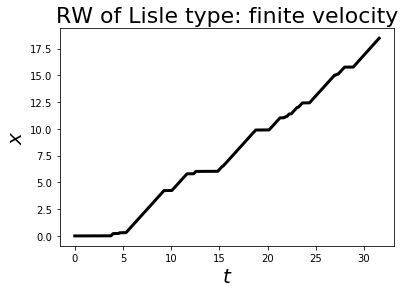
\includegraphics[width=0.5\textwidth,keepaspectratio]{lisle_rw.png}
	\caption{The \citet{Lisle1998} model with finite motion intervals. Motions appear as slanted lines, where the slope is the velocity $v$ of motion. These types of walkers show super-diffusion at short timescales and normal diffusion at long timescales.}
	\label{fig:lislewalk}
\end{wrapfigure}
I need to carefully investigate whether \citet{Gordon1972} did it too.
They imparted a finite duration to bedload motions instead of considering them instantaneous like Einstein. In this way they derived two stages of bedload diffusion.
This approach is closely related to the so-called persistent diffusion model \citep{Balakrishnan1988,VanDenBroeck1990}, the diffusion of a particle driven by dichotomous Markov noise \citep[e.g.][]{Horsthemke1984,Risken1989,Bena2006}. 
The mathematics were essentially developed by Takacs (1957).

It is obtained by the choice $g_1(x,t) = \delta(x) k_1 e^{-k_1 t}$ (rest) and $g_2(x,t) = \delta(x-vt)k_2 e^{-k_2 t} $ (motion).
Hence motions occur with velocity $v$ for a duration characterized by an exponential distribution with mean $1/k_2$, while rests occur for a duration characterized by an exponential distribution with mean $1/k_1$. 
We consider each of the extreme initial conditions in turn.

\subsection{Rest initial state}

If the process starts from rest, this means $\theta_1 = 1$ and $\theta_2=0$.
In this case the Laplace transforms are
\be \tg_1(\eta,s) = \frac{k_1}{k_1 + s}, \ee 
\be \tg_2(\eta,s) = \frac{k_2}{k_2 + \eta v + s }\ee
and
\be \tG_i(\eta,s) = \frac{1}{k_i}\tg_i(\eta,s).\ee
Plugging these into (\ref{eq:mw}) gives
\be \tilde{p}(\eta,s) = \frac{k + s + \eta v }{(k_1+s) \eta v  + (k+s)s },\ee
where $k = k_1 + k_2$. 
This inverts to 
\be \tilde{p}(x,s) = \frac{k(k+s)}{v(k_1+s)^2} \exp\Big[-\frac{s(k+s)}{v(k_1+s)}x\Big] + \frac{1}{k_1+s}\delta(x) .\ee
Using the property $ \El\{f(x+a);s\} = e^{as}\El\{f(x);s\}$ along with the transform of a modified Bessel function gives
\begin{multline}
p(x,t) = \delta(x) e^{-k_1 t} + \frac{k}{v}\exp\Big[-\frac{k_2x }{v} - k_1\Big(t-\frac{x}{v}\Big)\Big]\Theta(t-x/v)\\ 
\times \Big\{ I_0\Big(2\sqrt{\frac{k_1k_2x}{v}\big(t-\frac{x}{v}\big)}\Big) \\
\sqrt{\frac{k_2 v(t-x/v)}{k_1x}}I_1\Big(2\sqrt{\frac{k_1k_2x}{v}\big(t-\frac{x}{v}\big)}\Big) 
\Big\}
\end{multline}
for the distribution of $x$ at time $t$.
The non-dimensionalization proposed by Lisle is $\xi = k_+ x /v$ and $\tau = k_-(t-x/v)$.
In this notation the result appears as
\be p(\xi,\tau) = \frac{k_2}{v}\delta(\xi)e^{-\tau-k_1\xi/k_2} +  \frac{k}{v}e^{-\xi-\tau}\Theta(\tau)\Theta(\xi)\Big\{I_0\big(2\sqrt{\xi \tau}\big) +\frac{k_2}{k_1}\sqrt{\frac{\tau}{\xi}}I_1\big(2\sqrt{\xi\tau}\big) \Big\}\ee

\subsubsection{Analytical solution of moments from rest}
The first derivative gives 
\be \bra \tilde{x} \ket = vk_1 \frac{1}{s^2(k+s)}, \label{eq:restmean}\ee
while the second gives 
\be \bra \tilde{x}^2 \ket = 2 v^2  k_1 \frac{k_1+s}{s^3(k+s)^2}. \label{eq:rest2ndmoment}\ee
Therefore the mean follows from \ref{eq:lap2}:
\be \frac{k^2}{vk_1} \bra x \ket = e^{-kt} + kt -1, \ee
and the second moment follows from \ref{eq:lap3} and \ref{eq:lap4}:
\begin{align}
\frac{k^4}{2v^2 k_1}\bra x^2 \ket = k_1\Big[\frac{(kt)^2}{2}-kt + 1 - e^{-kt}\Big] + k_2 \Big[kt -2 + (kt+2)e^{-kt}\Big]
\end{align}
Manipulating the mean provides 
\be \frac{k^4}{2v^2 k_1} \bra x \ket^2 = k_1 \Big(\frac{1}{2} e^{-2kt} + \frac{(kt)^2}{2} + \frac{1}{2} + (kt-1)e^{-kt} - kt\Big) \ee
so the variance is 
\be \frac{k^4}{2v^2 k_1}\sigma_x^2 = k_1 \Big[\frac{1}{2}-\frac{1}{2}e^{-2kt} - kt e^{-kt}\Big]  + k_2 \Big[kt -2 + (kt + 2)e^{-kt}\Big].\ee
Taylor expanding shows asymptotic behavior
\be \sigma_x^2 \sim 
\begin{cases}
	 \frac{1}{3}k_1v^2 t^3, & t\rightarrow 0 \\
	 2\frac{k_1k_2 v^2}{k^3} t, & t \rightarrow \infty.
\end{cases} \label{eq:sim}\ee
There is a cross-over from ballistic to normal diffusion.

\subsubsection{Asymptotic solution of moments from rest}
The $t\rightarrow \infty$ behavior comes from expanding \ref{eq:restmean} and \ref{eq:rest2ndmoment} at $s\rightarrow0$ and transforming. 
The expansions are 
\be \bra \tilde{x} \ket \sim vk_1 \Big( \frac{1}{ks^2} - \frac{1}{k^2 s}\Big)\ee
\be \bra \tilde{x}^2 \ket \sim 2v^2k_1\Big(\frac{k_1}{k^2s^3} + \frac{k_2-k_1}{k^3s^2}\Big)\ee
giving 
\begin{align} \sigma_x^2 &\sim  \frac{2v^2k_1^2 t^2}{2k^2} + \frac{2v^2k_1(k_2-k_1)t}{k^3}  - \frac{v^2k_1^2 t^2}{k^2} + \frac{2v^2k_1^2t}{k^3} \\ \sigma_x^2&\sim 2\frac{k_1k_2 v^2}{k^3} t,\end{align}
in agreement with \ref{eq:sim}. This was tricky to figure out. You have to keep the constant term in the mean.
Similarly the $t\rightarrow 0$ behavior comes from expanding  \ref{eq:restmean} and \ref{eq:rest2ndmoment} at $1/s\rightarrow0$ and transforming.
The expansions are 
\be \bra \tilde{x} \ket \sim  \frac{vk_1}{s^3}\Big(1-\frac{k}{s}\Big)\ee
\be \bra \tilde{x}^2 \ket \sim \frac{2v^2k_1}{s^4}\Big(1+ [k_1-2k]\frac{1}{s}\Big)\ee
giving asymptotic variance (at $t\rightarrow 0$)
\be \sigma_x^2 \sim \frac{1}{3}k_1v^2 t^3 \ee
in agreement with  \ref{eq:sim}.
\subsection{Motion initial state}

Now I'll try using the opposite initial condition (the one chosen by \citet{Lisle1998}): $\theta_2 = 1$ and $\theta_1 = 0$.
In this case
\be \tilde{p}(\eta,s) = \frac{k+s}{v(k_1+s)\eta + (k+s)s},\ee
and a first inverse transform gives
\be p(x,s) = \frac{k+s}{v(k_1+s)} \exp\Big[-\frac{(k+s)s}{v(k_1+s)}x\Big],\ee
which is the same as the other case but without a delta function term at $x=0$.
This can be manipulated to 
\begin{align} p(x,t) &= \El^{-1} \Big\{ \frac{k+s}{v(k_1+s)} \exp\Big[-\frac{(k+s)s}{v(k_1+s)}x\Big] ; t\Big\} \\
&=  e^{-k_1 t}\El^{-1} \Big\{ \frac{k_2+s}{vs} \exp\Big[-\frac{(k_2+s)(s-k_1)}{vs}x\Big] ; t\Big\} \\
&= e^{-k_1 t -(k_2-k_1)x/v}\El^{-1} \Big\{ \frac{k_2+s}{vs} \exp\Big[\frac{k_1k_2}{vs}x - \frac{xs}{v}\Big] ; t\Big\}\\
&= e^{-k_1 t -(k_2-k_1)x/v}\El^{-1} \Big\{ \frac{k_2+s}{vs} \exp\Big[\frac{k_1k_2}{vs}x\Big] ; t-x/v\Big\} \\
&=  e^{-k_1 t -(k_2-k_1)x/v} \Big[ \El^{-1}  \Big\{ \frac{k_2}{vs} \exp\Big[\frac{k_1k_2}{vs}x\Big];t-x/v \Big\} + \El^{-1}  \Big\{ \frac{1}{v} \exp\Big[\frac{k_1k_2}{vs}x\Big];t-x/v \Big\} \Big] \\
&=  e^{-k_1 t -(k_2-k_1)x/v} \Big[\frac{k_2}{v} I_0\Big(2\sqrt{\frac{k_1k_2 x}{v}\big(t-\frac{x}{v}\big)}\Big) + \frac{1}{v}\El^{-1}\Big\{  \exp\Big[\frac{k_1k_2}{vs}x\Big] -1;t-x/v \Big\} + \frac{1}{v}\delta(t-x/v) \Big] \\ 
&=  e^{-k_1 t -(k_2-k_1)x/v} \Big[\frac{k_2}{v} I_0\Big(2\sqrt{\frac{k_1k_2 x}{v}\big(t-\frac{x}{v}\big)}\Big) + \frac{1}{v}\sqrt{\frac{k_1 k_2 x}{v (t-x/v)}}I_1\Big(2\sqrt{\frac{k_1k_2 x}{v}\big(t-\frac{x}{v}\big)}\Big) + \frac{1}{v}\delta(t-x/v) \Big].
\end{align}
A key property here was $e^{-ax}f(x) = \El^{-1}\{f(s+a);x\}$, and those in the appendix.
This type of math is not easy for me.
In the non-dimensional variables this becomes
\be p(\xi,\tau) = e^{-\tau-\xi}\Big[ \frac{k_2}{v} I_0(2\sqrt{\xi\tau}) + \frac{k_1}{v}\sqrt{\frac{\xi}{\tau}}I_1(2\sqrt{\xi\tau}) + \frac{k_1}{v} \delta(\tau)\Big].\ee
This appears totally aligned with \citet{Lisle1998}.
\subsubsection{moments having started in motion}
Taking derivatives (it's easier this time) gives 
\be \bra \tilde{x} \ket = v \frac{k_1 + s}{s^2(s+k)} \ee
\be \bra \tilde{x}^2 \ket = 2v^2 \frac{(k_1+s)^2}{s^3(k+s)^2}.\ee
Using \ref{eq:lap2} and \ref{eq:lap6} gives
\be \frac{k^2}{v}\bra x \ket = k_1 kt + k_2(1-e^{-kt}).\ee
Using \ref{eq:lap3}, \ref{eq:lap4}, and \ref{eq:lap5} gives
\be \frac{k^4}{2v^2}\bra x^2\ket = k_1^2 \frac{(kt)^2}{2} + k_1 k_2 \Big[2kt-2+2e^{-kt}\Big] + k_2^2 \Big[1-(1+kt)e^{-kt}\Big].\ee
Manipulating the mean to 
\be \frac{k^4}{2v^2}\bra x\ket^2 = k_1^2 \frac{(kt)^2}{2} + k_1 k_2\Big[\frac{1}{2}+ \frac{1}{2}e^{-2kt}-e^{-kt}\Big] + k_2^2\Big[kt -kte^{-kt}\Big]\ee
provides a variance
\be \frac{k^4}{2v^2k_2}\sigma_x^2 = k_1\Big[kt + (2+kt)e^{-kt} -2\Big] 
+ k_2\Big[\frac{1}{2} - \frac{1}{2}e^{-2kt} - kt e^{-kt}\Big].\ee
Expanding this reveals asymptotic behavior 
\be \sigma_x^2 \sim 
\begin{cases}
	\frac{1}{3}k_2v^2 t^3, & t\rightarrow 0 \\
	2\frac{k_1k_2 v^2}{k^3} t, & t \rightarrow \infty.
\end{cases} \label{eq:sim}\ee
The conclusion is initial condition does not affect the asymptotic scaling.
This is still super-diffusion $\sigma_x^2 \propto t^3$ crossing to normal diffusion $\sigma_x^2 \propto t$.
It only affects the coefficient of this scaling. 
\subsubsection{asymptotic approach to the moments starting in motion}
Same story exactly. Not very interesting.
\be \sigma_x^2 \sim 
\begin{cases}
	\frac{1}{3}k_2v^2 t^3, & t\rightarrow 0 \\
	2\frac{k_1k_2 v^2}{k^3} t, & t \rightarrow \infty.
\end{cases} \label{eq:sim}\ee
with no hiccups.
\subsection{Mixed initial state}
With an arbitrary mixed state the double transformed density is 
\begin{align}
\tilde{p}(\eta,s) &= \theta_1 \frac{k + s + \eta v }{(k_1+s) \eta v  + (k+s)s } + \theta_2\frac{k+s}{v(k_1+s)\eta + (k+s)s}\\
&=  \frac{k + s + \theta_1 \eta v }{(k_1+s) \eta v  + (k+s)s }
\end{align}
with the identity $\theta_1+\theta_2=1$.
\subsubsection{analytical approach to the moments in an arbitrary mixed state}
Taking one derivative gives
\be \partial_\eta \tilde{p}(\eta,s) = -v \frac{(\theta_2s + k_1)(k+s)}{[(k_1+s) \eta v  + (k+s)s]^2}, \ee
and a second gives
\be \partial_\eta^2 \tilde{p}(\eta,s) = 2v^2 \frac{(\theta_2s + k_1)(k+s)(k_1+s)}{[(k_1+s) \eta v  + (k+s)s]^3}, \ee
so the transformed first and second moments are 
\be \bra \tilde{x} \ket = v \frac{k_1 + \theta_2s}{s^2(k+s)}\ee
\be \bra \tilde{x}^2 \ket = 2v^2 \frac{(k_1 + \theta_2s)(k_1+s)}{s^3 (k+s)^2}.\ee
These expressions seem correct since $\theta_2=0$ and $\theta_2=1$ cases provide the earlier expressions.
Inverting the mean obtains
\begin{align} \frac{k^2}{v}\bra x \ket &= k_1 \Big[\theta_1 e^{-kt} + kt - \theta_1 \Big] + k_2 \theta_2 \Big[1-e^{-kt}\Big] \\
&= k_1 \Big[(1-\theta_2) e^{-kt} + kt + (\theta_2-1) \Big] + k_2 \theta_2 \Big[1-e^{-kt}\Big],
\end{align}
which still reduces to both earlier results.
After more work the second moment becomes
\begin{multline} \frac{k^4}{2v^2}\bra x^2 \ket = k_1^2 \Big[\frac{(kt)^2}{2} -kt + 1 - e^{-kt} + \theta_2\big\{k t -1 + e^{-kt}\big\}\Big] \\+ k_1k_2\Big[kt-2+(kt+2)e^{-kt} + \theta_2\big\{kt - kte^{-kt}\big\}\Big] \\+ k_2^2\theta_2\Big[1-(1+kt)e^{-kt}\Big]\end{multline}
which still reduces to earlier results.
Proceeding from here gets very difficult and messy. It's possible.
\subsubsection{asymptotic approach to the moments in an arbitrary mixed state}
Expanding the earlier expressions for $s \rightarrow \infty$ gives
\be \bra \tilde{x} \ket = v \Big[\frac{\theta_2}{s^2} + \frac{k_1-\theta_2 k}{s^3}-\dots\Big]
\ee
\be \bra \tilde{x}^2 \ket = 2v^2\Big[\frac{\theta_2}{s^3} + \frac{k_1\theta_2 + k_1 - 2k\theta_2}{s^4}+\dots\Big]\ee
transforming to 
\be \bra x \ket \sim v \Big[\theta_2 t + (k_1-\theta_2 k)\frac{t^2}{2}\Big]
\ee
\be \bra x^2 \ket \sim 2v^2 \Big[\frac{\theta_2t^2}{2} + \frac{t^3}{3!}(k_1\theta_2 + k_1 - 2k\theta_2)\Big].
\ee
The square of the mean is $\bra x \ket^2 \sim v^2\theta_2^2 t^2 + v^2\theta_2(k_1-\theta_2 k)t^3$,
so the variance is (as $t \rightarrow 0$)
\be \sigma_x^2 \sim v^2 \theta_1 \theta_2 t^2 + \frac{1}{3}(\theta_1 k_1 + \theta_2 k_2)v^2t^3.\ee
This reproduces both earlier results and explains the link between \citet{Lisle1998} and my other investigations with the dichotomous Markov noise \citep[e.g.][]{Horsthemke1984, Bena2006}.
\subsection{Summary of Lisle process}
This process supports two stages of diffusion: short-time super-diffusion and long time normal-diffusion.
The results are all correct and verified by simulations in figure \ref{fig:lislesims}.
\begin{figure}[h]
	\centering
	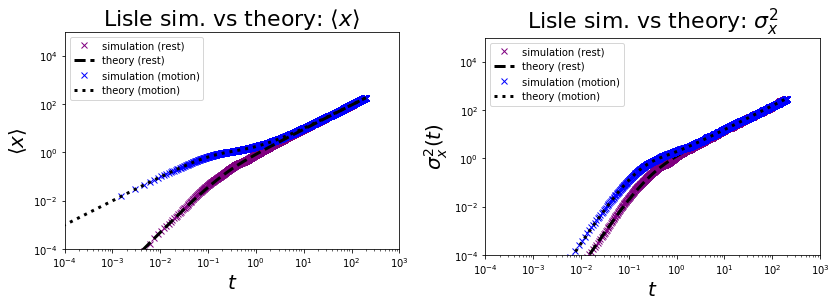
\includegraphics[width=\linewidth,keepaspectratio]{combo1.png}
	\caption{Variance and mean scaling compared to numerical simulations}
	\label{fig:lislesims}
\end{figure}

The two stages of diffusion and their asymptotic behavior are indicated in figure \ref{fig:lisledif}. The initial ballistic diffusion is at least $\sigma_x^2 \propto t^2$ and at most $\sigma_x^2 \propto t^3$, and the crossover to normal diffusion occurs around $\text{max}\{1/k_1,1/k_2\}.$
\begin{figure}[h]
	\centering
	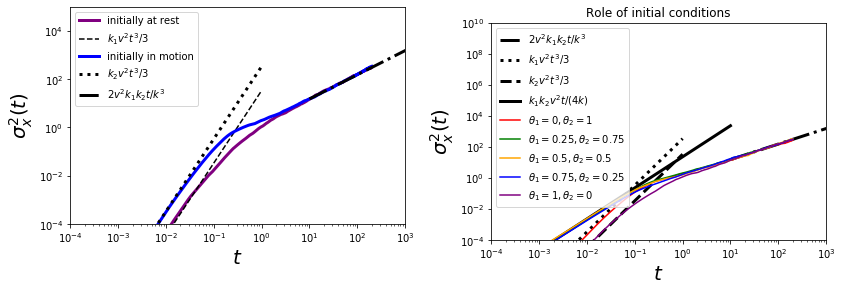
\includegraphics[width=\linewidth,keepaspectratio]{combo2.png}
	\caption{Scaling behavior of variance. Left panel shows pure initial conditions while the action-packed right panel shows mixed initial conditions. Mixed initial express a $\sigma_x^2 \propto t^2$ term. }
	\label{fig:lisledif}
\end{figure}

\section{Heavy-tailed resting time in a two-state walk}
Set $\psi_1(t) = A_\alpha t^{-\alpha}$ for $t\geq t_\alpha$.
$A_\alpha = (\alpha-1)t_\alpha^{\alpha-1}$ \citep[e.g.][eq. 12]{Weeks1996}.
Consider everything else the same as the \citet{Lisle1998} process.
The laplace transform of $\psi_1(t)$ is
\be \tilde{\psi}(s) = A_\alpha s^{\alpha-1}\Gamma(1-\alpha,st_\alpha).\ee
The incomplete gamma function is defined by 
\be \Gamma(q,x) = \int_x^\infty t^{q-1}e^{-t}dt.\ee
There's a need to expand this at small arguments.
Crucially, \citet{Weeks1996} did not use the standard Pareto distribution notation.

\subsection{$t\rightarrow \infty$ expected behavior}
$\alpha<1/2$ implies subdiffusion. $1/2<\alpha<2$ implies superdiffusion, $\alpha>2$ implies normal diffusion.

\section{A new generalization: Randomly stopped Lisle process}

Consider the choice $\psi_1(t) = k_1e^{-k_1t}$, $f_1(x,t)=\delta(x)$, $\psi_2(t) = k_2e^{-k_2t}$, and 
\be f_2(x,t|T) = \delta(x-vt)\Theta(T-t) + \delta(x)\Theta(t-T).\ee
This describes a \textit{randomly stopped} variant of the Lisle process.
When $t>T$, the motion state becomes a second rest state: the motion is turned off.
In this case, $g_1(\eta,s) = \frac{k_1}{k_1+s}$ and $G_1(\eta,s) = g_1(\eta,s)/k_1$ as before, while
\be g_2(\eta,s|T) = \frac{k_2}{k_2+s}e^{-(k_2+s)T} + \frac{k_2}{k_2 + \eta v + s}\Big(1-e^{-(k_2 + \eta v + s)T}\Big)\ee
and $G_2(\eta,s|T) = g_2(\eta,s|T)/k_2$.
You can maybe solve this conditional to $T$ to obtain $p(x,t|T)$.
Then inputting a distribution for the trapping time $T$, the over-all distribution will be $p(x,t) = \int dT p(x,t|T)f(T)$.

Assuming the walker starts at rest, the double transformed probability is
\be \tilde{p}(\eta,s) = \ee


\section*{Appendix: Laplace transforms}
This is just a reference of useful Laplace transforms for these types of studies.
\be \El\Big\{\frac{1}{s^{k+1}};s\Big\} = \frac{t^k}{k!}; \label{eq:lap1}\ee

\be \El^{-1}\Big\{p^{-2}(p+a)^{-1};x\Big\} = \frac{1}{a^2}(e^{-ax}+ax-1),\label{eq:lap2}\ee
\citep[][2.1.2.33]{Prudnikov1986};
\be \El^{-1}\Big\{p^{-2}(p+a)^{-2};x\Big\} = \frac{1}{a^3}[ax - 2 + (ax+2)e^{-ax}],\label{eq:lap3}\ee
\citep[][2.1.2.49]{Prudnikov1986};
\be \El^{-1}\Big\{p^{-3}(p+a)^{-2};x\Big\} = \frac{1}{a^4}\Big[\frac{(ax)^2}{2} - 2ax - (ax+3)e^{-ax} + 3\Big], \label{eq:lap4}\ee
derived from the previous result using the differentiation property;
\be \El^{-1}\Big\{p^{-1}(p+a)^{-2};x\Big\} = \frac{1}{a^2}\Big(1 -(1+ax)e^{-ax}\Big), \label{eq:lap5}\ee
\citep[][2.1.2.47]{Prudnikov1986};
\be \El^{-1}\Big\{p^{-1}(p+a)^{-1};x\Big\} = \frac{1}{a}(1-e^{-ax}),\label{eq:lap6}\ee
\citep[][2.1.2.31]{Prudnikov1986};
\be\El^{-1} \{e^{as}\tilde{f}(s);x\} = \El^{-1}\{\tilde{f}(s);x+a\},\label{eq:lap7}\ee
the shifting property;
\be \El^{-1}\big\{\frac{1}{s^\nu}\exp(a/s);t\} = \Big(\frac{t}{a}\Big)^{(\nu-1)/2}I_{\nu-1}\big(2\sqrt{a t}\big), \label{eq:lap8}\ee
valid for $\nu>1$ from \citep[][2.2.2.1]{Prudnikov1986};
\be \El^{-1}\{e^{a/p}-1;x\} = \sqrt{\frac{a}{x}}I_1(2\sqrt{ax}),\label{eq:lap9}\ee
and \citep[][2.2.2.8]{Prudnikov1986}.
All of these Laplace transforms are verified from Wolfram Alpha so I expect no typos.
Finally,
\be \El\Big\{\frac{a}{bs+c};s\Big\} = \frac{a}{b}e^{-cx/b}\label{eq:lap10}\ee
and
\be \El\Big\{\frac{as}{bs+c};s\Big\} = \frac{a}{b}\Big[\delta(x) - \frac{c}{b}e^{-cx/b}\Big].\label{eq:lap11}\ee
The Laplace transform of a first derivative is 
\be \El\{f'(t)\} = s\tilde{f}(s)-f(0),\ee
while a second derivative is 
\be \El\{f''(t)\} = s^2 \tilde{f}(s) - sf(0) -f'(0).\ee
\section*{Appendix: Asymptotics of stable laws}
When a resting time distribution $\psi(t)$ has divergent moments, the behavior of its Laplace transform $\tilde{\psi}(s)$ for $s\rightarrow0$ cannot be analyzed by simply expanding the exponential in its definition for small $s$ as in 
\be \tilde{\psi}(s) \sim \int_0^\infty \{1-st + (st)^2/2 + \dots \} \psi(t),\ee
since the moments of $t$ involved in this expression are divergent. 
Instead, there is a different way (outlined around \citet{Weiss1994} eq 2.95) leveraging the asymptotic form of $\psi(t)$ for $t\rightarrow \infty$:
\be \psi(t) \sim  A t^{-\alpha-1}.\ee
Writing (using the normalization property of $\psi(t)$)
\be \tilde{\psi}(s) = 1 - (1- \tilde{\psi}(s)) = 1 - \int_0^\infty dt (1-e^{-st})\psi(t) \ee
and setting $\tau = st$ gives
\be \tilde{\psi}(s) = 1 - \frac{1}{s} \int_0^\infty d\tau (1-e^{-\tau})\psi\big(\frac{\tau}{s}\big).\ee
Clearly this integral is dominated by the asymptotic behavior of $\psi(t)$:
\be \tilde{\psi}(s) \sim 1 - B s^\alpha \ee
This is an important result for analyzing asymptotics of random walks involving power-law pausing time densities.
The coefficient $B$ is obtained (if necessary) by integrating the asymptotic power law using its coefficients and small-time cutoff.
Such an argument is essential to the paper of \citet{Weeks1998}. They give $B$ in terms of an incomplete Gamma function, which I could do if I wanted.

\section*{Appendix: Modified Bessel functions of the first kind}
A cool property is 
\be I_n(x) = T_n\Big(\frac{d}{dx}\Big)I_0(x)\ee
where $T_n$ is a Chebyshev polynomial of the first kind:
\begin{align}
T_0(x) &= 1 \\
T_1(x) &= x \\
T_2(x) &= 2x^2 -1 \\
&\vdots
\end{align}
This is available at \url{http://mathworld.wolfram.com/ModifiedBesselFunctionoftheFirstKind.html}.
In particular, 
\be I_1(x) = I_0'(x).\ee
The large $x$ expansion ($x\gg | \nu^2-1/4|$) of the modified Bessel function of the first kind is 
\be I_\nu(x) \approx \frac{e^x}{\sqrt{2\pi x}}\Big(1 + \frac{(1-2\nu)(1+2\nu)}{8x} + \dots \Big)\ee
while the small $x$ expansion ($0\leq x \leq \sqrt{\nu+1}$) is
\be I_\nu(x) = \frac{1}{\Gamma(\nu+ 1)}\Big(\frac{x}{2}\Big)^\nu.\ee
These are from \url{https://pdfs.semanticscholar.org/48dc/ca3cffb78de80ab37b84a992379c2f30bdda.pdf}.
The recurrence relations are
\be I_{\nu-1}(x) - I_{\nu+1}(x) = \frac{2\nu}{x}I_\nu(x)\ee
\be I_{\nu-1}(x) + I_{\nu+1}(x) = 2\frac{d}{dx}I_\nu(x).\ee
\bibliography{biblio}
\end{document}



